%
% tests.tex
%
% Copyright (C) 2021 by SpaceLab.
%
% TTC Documentation
%
% This work is licensed under the Creative Commons Attribution-ShareAlike 4.0
% International License. To view a copy of this license,
% visit http://creativecommons.org/licenses/by-sa/4.0/.
%

%
% \brief Tests chapter.
%
% \author Gabriel Mariano Marcelino <gabriel.mm8@gmail.com>
%
% \institution Universidade Federal de Santa Catarina (UFSC)
%
% \version 1.2.0
%
% \date 2021/01/16
%

\chapter{Tests} \label{ch:tests}

This...

\section{RF Signal Frequency}

\subsection{Beacon}

\begin{itemize}
    \item Target: 145,9 MHz
    \item Measurement: $\cong$ 145,9 MHz
\end{itemize}

\begin{figure}[H]
    \begin{center}
        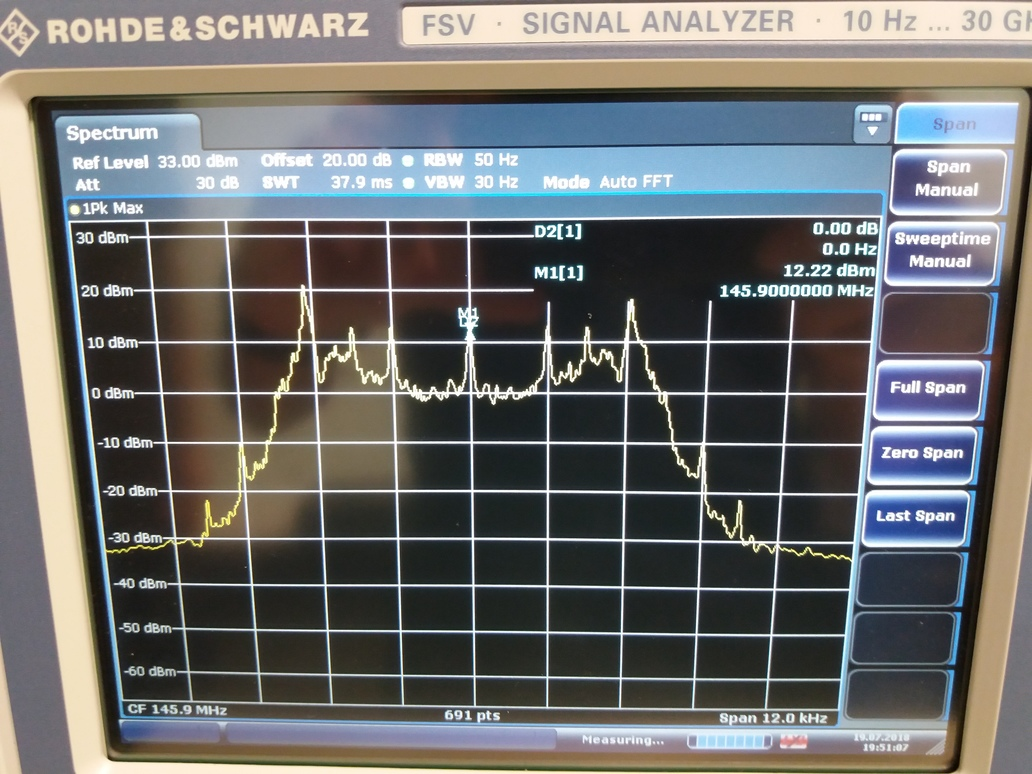
\includegraphics[width=0.8\textwidth]{figures/tests/beacon_frequency.jpg}
        \caption{Beacon output frequency.}
        \label{fig:beacon-frequency}
    \end{center}
\end{figure}

\subsection{Downlink}

\begin{itemize}
    \item Target: 437,9 MHz
    \item Measurement: $\cong$ 437,9 MHz
\end{itemize}

\begin{figure}[H]
    \begin{center}
        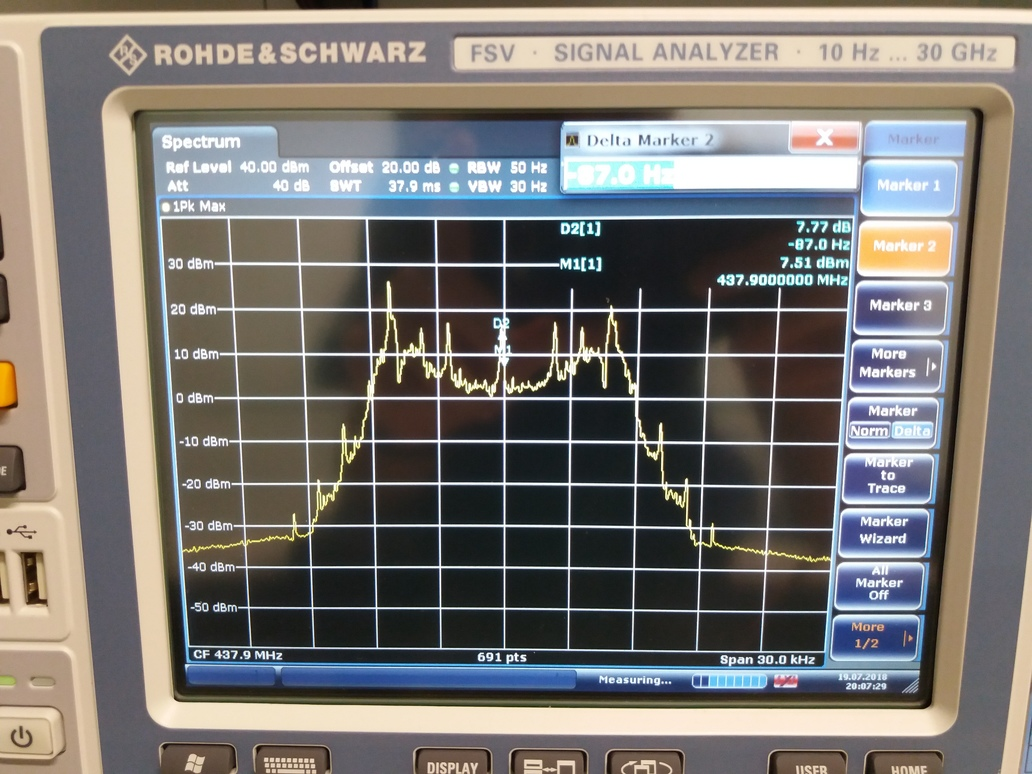
\includegraphics[width=0.8\textwidth]{figures/tests/downlink_frequency.jpg}
        \caption{Downlink output frequency.}
        \label{fig:downlink-frequency}
    \end{center}
\end{figure}

\section{RF Signal Power}

\subsection{Beacon}

\begin{itemize}
    \item Target: 30 dBm
    \item Measurement: $\cong$ 22 dBm (+3 dBm including the cable and connectors loss)
\end{itemize}

\begin{figure}[H]
    \begin{center}
        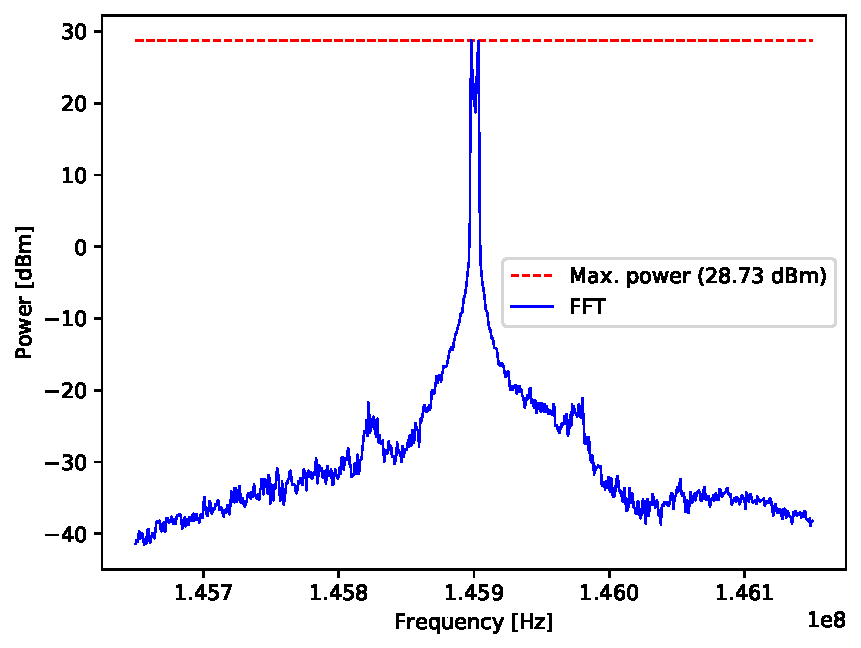
\includegraphics[width=0.8\textwidth]{figures/tests/beacon_output_power.pdf}
        \caption{Beacon output power.}
        \label{fig:beacon-output-power}
    \end{center}
\end{figure}

\subsection{Downlink}

\begin{itemize}
    \item Target: 30 dBm
    \item Measurement: $\cong$ 27 dBm (+3 dBm including the cable and connectors loss)
\end{itemize}

The output power of the downlink radio can be seen in \autoref{fig:downlink-frequency}.

\section{Harmonics}

\subsection{Beacon}

\begin{figure}[H]
    \begin{center}
        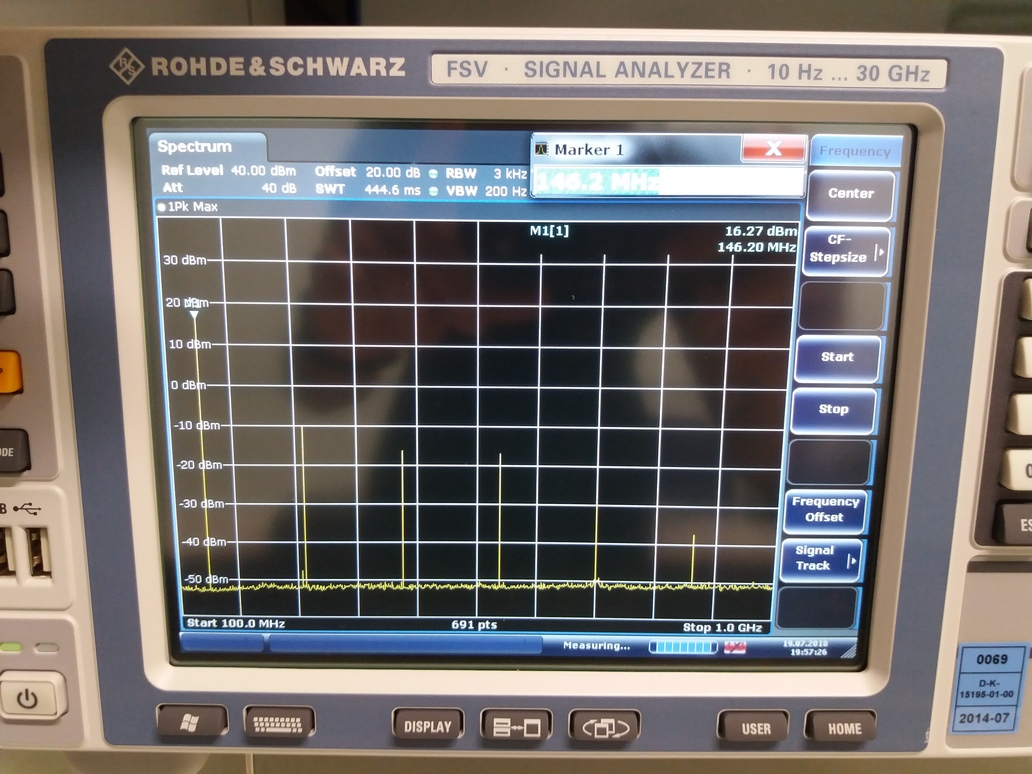
\includegraphics[width=0.8\textwidth]{figures/tests/beacon_harmonics.jpg}
        \caption{Beacon signal harmonics.}
        \label{fig:beacon-harmonics}
    \end{center}
\end{figure}

\begin{figure}[H]
    \begin{center}
        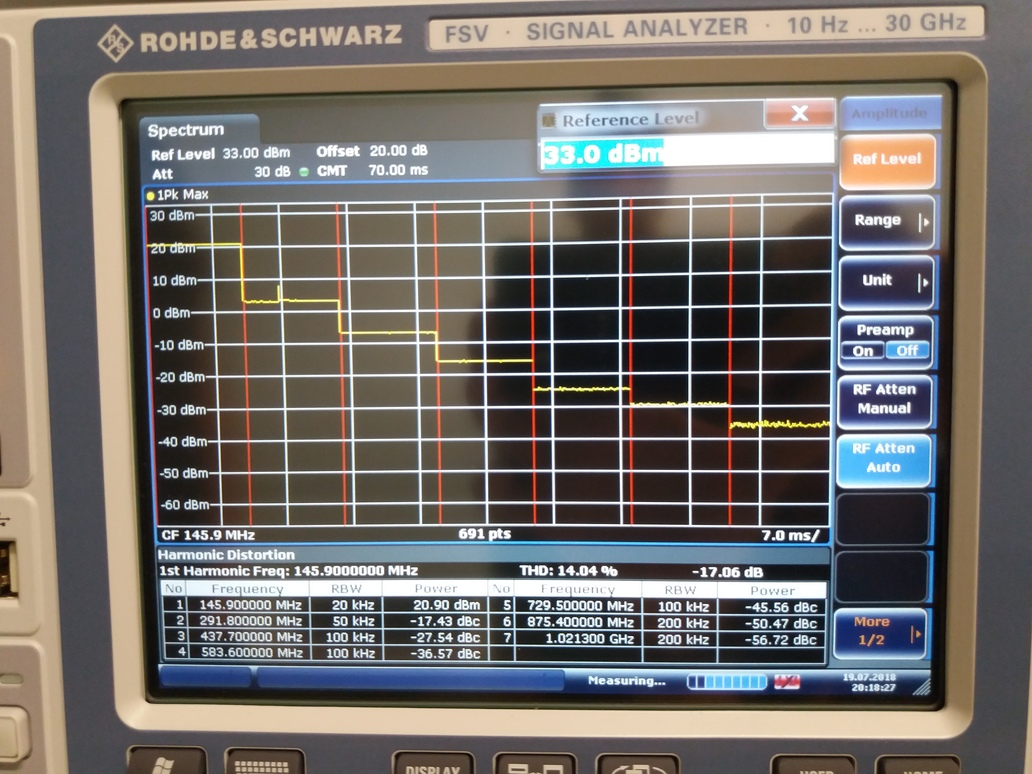
\includegraphics[width=0.8\textwidth]{figures/tests/beacon_harmonics_analysis.jpg}
        \caption{Analysis of the beacon signal harmonics.}
        \label{fig:beacon-harmonics-analysis}
    \end{center}
\end{figure}

\subsection{Downlink}

\begin{figure}[H]
    \begin{center}
        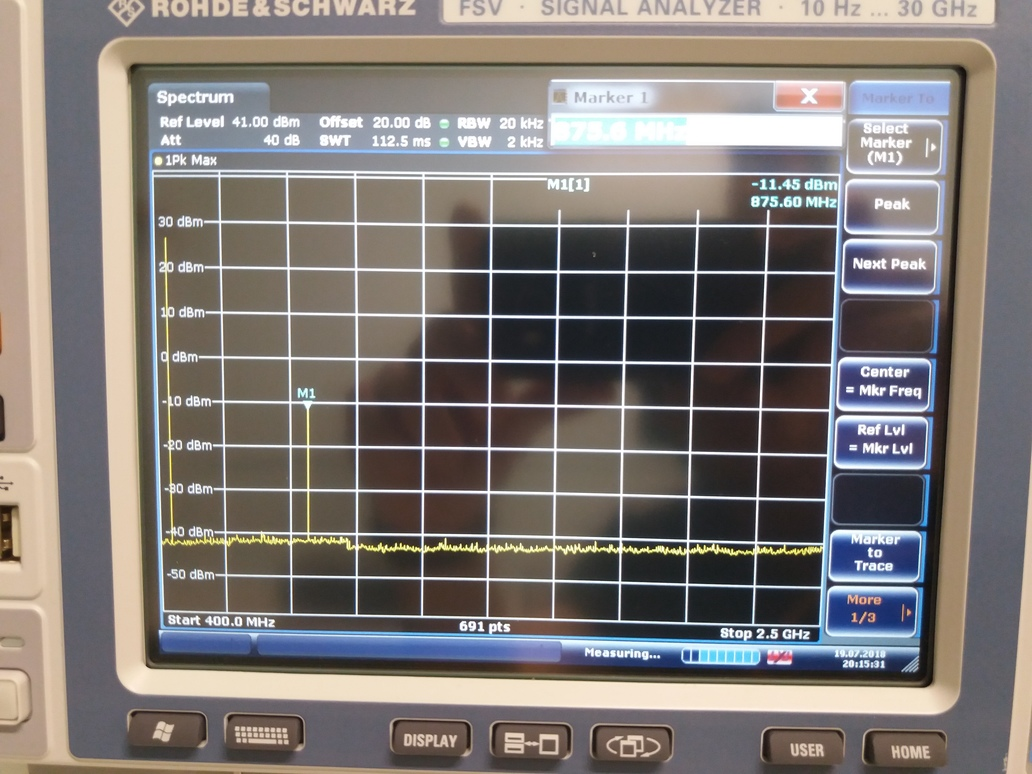
\includegraphics[width=0.8\textwidth]{figures/tests/downlink_harmonics.jpg}
        \caption{Downlink signal harmonics.}
        \label{fig:downlink-harmonics}
    \end{center}
\end{figure}
